\chapter{State of the Art}\label{chap:state-of-the-art}

A modular robotics is a way to build robots consisting of \emph{modules}. In
context of this paper, modules are rather high-level pieces with a certain level
of self-control instead of low-level components like individual actuators or
sensors. It might even make sense to talk about modules as individual robots,
which are used to build bigger robots. The modules have usually a limited set of
capabilities -- often the functionality is so primitive, the modules cannot
perform useful tasks on their own. However, when we join multiple modules, they
can cooperate and, therefore, new capabilities of the system as a whole emerge.
This idea probably first appeared in the work by
\textcite{DBLP:conf/icra/FukudaK90}, where they introduced CEBOTs (Cellular
Robotic System).

\section{Taxonomy of Existing Modular Robots}

Since the era of CEBOTs, many more projects followed and the research area split
into two: smart (or programmable) matter and modular robotics. The smart matter
aims at building very simple modules leveraging physical and chemical principles
(imagine artificial atoms) in order to create blob of modules, which can
reassemble into a different, usually solid, object based on an external input.
Contrary, the modular robotics aims at building more complex modules, which are
able of sophisticated self-organization (imagine artificial cells), which can
form usually highly dynamic robots that can autonomously move and interact with
their environment. Smart matter also aims at sub-millimeter modules, modular
robotics aims at sub-centimeter modules \cite{DBLP:conf/ieeealife/Christensen07,
1285597}. In the rest of this paper, we will omit smart matter and focus
exclusively on modular robots.

What distinguishes modular robots from swarm robotics is the ability of the
modules to mechanically connect and inherently form a larger robot. The
connection can be performed externally, e.g., by an operator, or the modules can
connect on their own. Even the trend is to build self-reconfigurable robots,
there are occasionally some exceptions, e.g., PetRo
\cite{DBLP:conf/ro-man/Salem14}.

There have been many more or less successful projects of self-reconfigurable
modular robots since the CEBOTs. The projects feature various designs approaches
from the capabilities of individual modules to the topology in which the modules
connect. Most of the projects used metamorphic modules, i.e., there is only a
single or a few types of modules in the system. We consider the following list
as a nice representable sample of the various designs: Fracta
\cite{DBLP:conf/icra/MurataKK94}, Molecule \cite{DBLP:conf/icra/KotayRVM98},
Polybot \cite{DBLP:conf/icra/YimDR00}, M-TRAN
\cite{DBLP:conf/icarcv/KurokawaKYTMK02}, Atron
\cite{DBLP:conf/iros/JorgensenOL04}, Superbot \cite{DBLP:conf/iros/SalemiMS06},
Molecube \cite{DBLP:journals/trob/ZykovMDL07}, Roombots
\cite{DBLP:conf/icra/SprowitzBDI09}, Symbricator
\cite{DBLP:journals/corr/abs-1109-2288}, SMORES \cite{DBLP:conf/iros/DaveyKY12},
M-Blocks \cite{DBLP:conf/iros/RomanishinGR13}, ModRED
\cite{DBLP:journals/ras/BacaHDND14}, HyMod \cite{DBLP:conf/dars/ParrottDG16} and
Omni-Pi-tent \cite{DBLP:conf/taros/PeckTT19}.

\textcite{4141032} distinguishes three categories of the robots based on the
topology in which they connect. Each category has its own specific problems of
control and makes some tasks easier than other:

\paragraph{Lattice architecture} have its modules arranged in regular 3D grid --
e.g., a cube or hexagonal grid. The modules are tightly packed together. Typical
examples of such architectures are M-Blocks \cite{DBLP:conf/iros/RomanishinGR13}
and Atron \cite{DBLP:conf/iros/JorgensenOL04}. The regular grid makes it easier
to create a reconfiguration schedule and execute in parallel (for more details
see Subsection \todo{ref}). However, reconfiguration is usually the only option
for locomotion of such system, and, therefore, lattice architectures do not
yield highly dynamic systems.

\paragraph{Chain architecture} have its modules connected in a string or
possibly in a tree. Typical examples of such architectures are Polybot
\cite{DBLP:conf/icra/YimDR00} and Molecubes
\cite{DBLP:journals/trob/ZykovMDL07}. This architecture allows for easy
formation of limbs and arms, therefore, these robots usually interact well with
the environment. Also even very simple controllers yield locomotion (via
snake-like movements (see Subsection \todo{ref} for more details). The chains
can also form space-filling curve, therefore, e.g., Molecubes, can form a
lattice-like structures, while the underlying structure is linear.

\paragraph{Hybrid architecture} allows for both arrangements of modules,
therefore combines the advantages of both, possibly at the cost of increased
complexity. Examples of such robots are M-TRAN~III
\cite{DBLP:journals/ijrr/KurokawaTKKHM08}, Roombots
\cite{DBLP:conf/icra/SprowitzBDI09}, SMORES \cite{DBLP:conf/iros/DaveyKY12},
HyMod \cite{DBLP:conf/dars/ParrottDG16} and Omni-Pi-tent
\cite{DBLP:conf/taros/PeckTT19}. We can perceive that the most recent trend is
to build hybrid architectures. Especially SMORES are designed to be able to
replicate arrangements of the other platforms, thus be as versatile as possible
\cite{DBLP:conf/iros/DaveyKY12}.

On top of the locomotion provided by the the inter-module interaction, some
systems feature locomotion of the individual modules - e.g, by providing wheels
(SMORES, HyMod) or tracks (Symbricator), which further makes the reconfiguration
problem easier by allowing the modules to move on their own in the space without
interaction with the rest of the modules. A good example of such solution is
work by \textcite{DBLP:journals/ral/LiuWY19}.

\section{Challenges of Modular Robots}

There are many common challenges of modular robotics and the robotics in
general. This challenges were nicely summarized recently in blog post by
\textcite{locklin_2020}. Most of the challenges can be characterized by shifting
the robots from single purpose devices used in industrial automation, which
follow a preprogrammed path ignoring any environment around them, to autonomous
devices which can move in and interact with environment and adapt to its
changes. The challenges includes problems like motion planning (how to get from
point A to point B and avoid obstacles), continuous mapping of the environment,
scene understanding, and affordance discovery (predicting how the object will
behave when the robot interacts with it).

In the rest of this paper, we will focus only on the challenges specific to
metamorphic robots. We will also deliberately omit the challenges of mechanical
and electrical design of such robots. We will only slightly touch them in
Section \ref{sec:mixed-challenges}.

Let us introduce the challenges and illustrate them on a simple case. Suppose
there is a robot composed out of the modules in a simple environment. See figure
\ref{fig:arena} for illustration of the environment. There are two elevated
ramps. On one of them, there is red cube. The robot is supposed to move the cube
from one ramp to another. There is also a power socket after a narrow passage.
The modules do not have enough energy to complete the whole task.

\begin{figure}[!t]
    \centering
    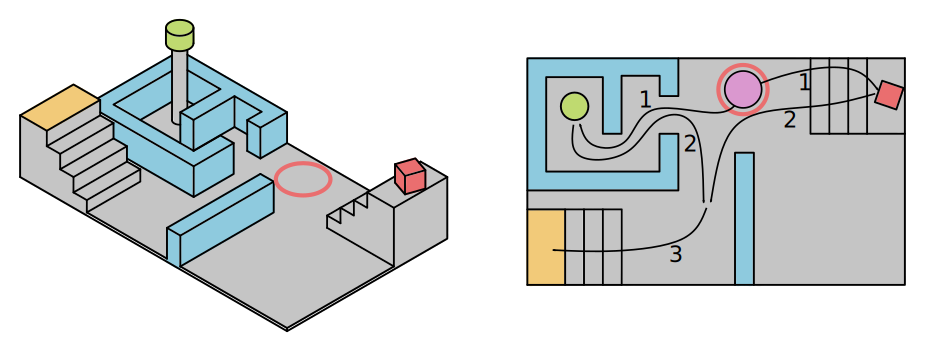
\includegraphics[width=0.7\textwidth]{figures/arena.jpg}
    \caption{The example environment for illustration of various challenges of
    self-reconfigurable robots.}
    \label{fig:arena}
\end{figure}

Once the robot is given the task, \footnote{Note, that for our purposes we omit
the translation step from "move the cube" to having a precise program saying
move to point A, grab a cube, move to point B, release the cube. We omit it as
we consider the translation as an open general problem of robotics.} we expect
it to find a plan to fullfil the task.

One of the possible solution is to first split in half and form two robots --
one will go to harvest energy, the second one will go and grab the cube. Then
then will join again on the way to the second ramp and share power. To do so,
the energy harvesting robot reconfigures into and energy efficient configuration
for locomotion and moves toward the narrow passage. Before the passage, it
reconfigure itself into a snake and passes it. Then it forms an arm and reaches
the power socket to charge itself. Meanwhile, the other robot moves towards the
first ramp. When it reaches the ramp, it changes shape so it can crawl the ramp
ramp and to grab the red cube cube. Then it returns and reunions with the energy
harvesting robot. They form a single robot and share the harvested power. During
climbing the other ramp, one of the modules in the systems stops responding,
therefore, however, the robot still continues to operate -- it just moves
slower. Before reaching the top of the ramp, the robots falls. It survives by
breaking inter-module connections to prevent module damage. The robots
reassembles and finishes the task.

Other possible solution (more suitable for cell-like robots, e.g., ATRON) is to
move in a \say{liquid blob of mass} which surrounds the cube and nudges it in
the desired direction.

In this simple example, we can identify several challenges typical for
self-reconfigurable robots. The first, obvious one, is \emph{planning
challenge}. The robot has to analyze the problem and figure out how to leverage
its ability to change shape to fulfill the task. The second challenge is the
challenge of \emph{locomotion} of the whole group of robots. Even the individual
modules can have wheels to move themselves, it is desirable to move in blocks as
new locomotion capabilities will emerge -- e.g. individual modules are not able
to climb stairs, but a system of them is. The next challenge is the
\emph{reconfiguration challenge}. This one is straightforward -- the robots have
to have an algorithm to compute reconfiguration plan to change shape. To
actually locomote, compute and schedule the reconfiguration we are facing the
\emph{control challenge}. We have to be able to control large number of modules
in a synchronized manner and ideally leverage all their computational potential.
All of the above should be designed in fault-tolerant way otherwise the large,
complex system will certainly fail. Also, the system has backed by solid
hardware and software solutions, which presents the \emph{mixed hardware and
software challenge}.

In the following section, we will discuss state-of-the-art for each of the
challenges individually.

\section{Planning Challenge}

For the purposes of this thesis, we consider planning for modular robots as an
effort to leverage the shape-changing ability of the self-reconfigurable robots
to fulfill tasks as efficient as possible and to adapt to an unknown or changing
environment. Note that planning often denotes also reconfiguration or locomotion
in the literature. For brevity, we also exclude work dealing with planning for a
single robot.

Despite we presented number of projects, nearly none of them deals with
planning. Instead, they focus rather on low-level control (locomotion and
reconfiguration), which we will cover in the later sections. To our knowledge,
there are two research groups that presented results in the area of high-level
planning of self-reconfigurable robots: SMORES and Symbricator.

There are several publications dealing with high-level planning for SMORES.
\textcite{DBLP:journals/arobots/JingTYK18} present a automata-based planner
(extension of their previous work \cite{DBLP:conf/ijcai/JingTYK17}), which takes
a task objective written in a \emph{Structured English}
\cite{DBLP:conf/iros/FinucaneJK10}. Their planner leverages a library of
handcrafted configurations. Each configuration have a set of properties and a
set of associated low-level controllers, which can perform single high-level
task -- e.g., move forward. The planner simply switches between those
configurations and controllers to achieve the specified goal. The switching is
based on a finite automaton. The automaton is synthesized from a set of formulas
in linear temporal logic (LTL) using an approach presented in
\cite{DBLP:journals/trob/Kress-GazitFP09}. The formulas come from the task
objective and additional constraints of the individual library configurations.
Note, that this approach is not brand new -- it was already introduced in
\cite{DBLP:conf/iros/CastroKK11} for CKBots, but work by
\textcite{DBLP:journals/arobots/JingTYK18} we just discussed, makes the approach
more robust and they present much more challenging experiments.

There is also work by \textcite{DBLP:conf/icra/TosunDJKCY18} on planning for
SMORES. They use a similar approach leveraging a library of hand-crafted
configuration as \cite{DBLP:journals/arobots/JingTYK18}. However, they extend
the system with \emph{environment augmentation modules} (just like
\cite{DBLP:conf/rss/PetersenNW11}) -- basically a passive modules serving as
building blocks for bridges and ramps, that can be used to augment the
environment, hence making fulfilling the objective easier for the robots.

Both of the presented approaches for SMORES use an external environment feedback
in the form of cameras with environment objects being tagged by black and white
patterns \cite{DBLP:journals/scirobotics/JingTYKC18}.

\textcite{DBLP:conf/syscon/LeviMRKVSLC14} take a different point of view on
planning for Symbricator. They focus and discuss mainly long-term plans for a
robotic system. Therefore, they propose that the planners should first focus on
the survival of the systems first (e.g., charging itself), and then, when
survival is guaranteed, the system should perform given tasks. Their
contribution lies in introduction of the \emph{SOS cycle}
(swarm-organism-swarm). In the cycle, the modules should first discover the
environment on their own (e.g., map it and locate power sources), then they
share the gathered information about environment. Then the modules assemble
together and fullfil a task. Once the task is completed (or failed), the modules
disassemble and the cycle repeats. In \cite{DBLP:conf/syscon/LeviMRKVSLC14},
they present advances on individual phases of the cycle (locomotion,
self-assembly, environment mapping). They also introduced concept of global
motion planning in \cite{DBLP:conf/icra/VonasekSKP13} using RRT
(rapidly-exploring random tree). This is an extension of the previous work
\cite{DBLP:conf/taros/VonasekKP12} by motion primitives -- a controllers for
specific configurations just like in the case of high-level planning for SMORES
\cite{DBLP:journals/arobots/JingTYK18}.

\section{Challenge of Reconfiguration}

There is a variety of work dealing with the reconfiguration problem. The work
differs by problem specification, used approaches and a mathematical model of a
robotic system.

Most of the work considers reconfiguration from given initial configuration to
given target configuration on chain or hybrid module types. The expected output
of the reconfiguration is a sequence of connect/disconnect operations and joints
movements to perform in order to reach the target configuration. Since all the
movements take time to complete and consume energy, it is desirable to find the
shortest reconfiguration sequence. Also, it is highly beneficial if the
reconfiguration plan can be computed in distributed manner to leverage the
computation power of the individual modules.

Exploration of the state-space of the system is a straightforward approach.
However, as \textcite{DBLP:journals/jfr/ChirikjianPE96} showed, the number of
possible configurations grows exponentially, therefore, direct explorations is
infeasible even for small systems. \textcite{DBLP:conf/iros/AsadpourASI09}
showed edit distance heuristics, that can improve performace of the search and,
therefore, increase size of the configuration which is manageable by this
approach. \textcite{DBLP:conf/monterey/BaarirHKR10} tackle the problem of large
state-spaces by using a symbolic representations inspired from software model
checking. All the work above demonstrates the results on MTRAN-like modules.

Since the modules in a system are from the reconfiguration point of view
indistinguishable from each other, we should treat isomorphic configuration as
the same. There are some advances in this area leveraging specific properties of
the robotic systems presented in \textcite{DBLP:journals/ijrr/ParkCTY08},
\textcite{DBLP:conf/iros/AsadpourASI09} and
\textcite{DBLP:journals/ras/TaheriMAP16}.

One of the most interesting results in reconfiguration is done by
\textcite{DBLP:journals/ras/HouS14}. They introduce a model of robotic system
called a \emph{connector graph}). They show that the problem of finding the
shortest reconfiguration plan between two connector graphs is NP-complete. They
provide an exponential distributed algorithm and also an approximative
distributed algorithm running in polynomial time for the problem. Since
connector graphs capture only topology, this approach produces only
connect/disconnect actions. Hence, it might produce a plan which is not
collision-free and cannot be executed due to physical limitations. Such plans
are suitable for robots with good self locomotion (e.g., SMORES) but hard-to-use
in a system lacking individual modules locomotion (e.g., M-BLOCKS or M-TRAN).
When the modules can move on their own, they can simply disconnect from the
system, move to the target location, and connect there as presented in
\cite{DBLP:journals/ral/LiuWY19}.

As the reconfiguration on connector graphs is NP-complete,
\textcite{DBLP:journals/pcs/GorbenkoP12} present a solution to the
reconfiguration via reduction to the Boolean satisfiability problem (SAT).

Other results aim at finding a feasible plan rather than the shortest one. To
name a few, \textcite{10.1117/12.360345} use the divide and conquer approach.
\textcite{DBLP:conf/icra/HouS08} present a reconfiguration emerging from local
behaviors in tree configurations. \textcite{DBLP:journals/ral/LiuWY19} use
dynamic programming for reconfiguration between tree configurations.

\textcite{DBLP:conf/iros/ButlerBR01} present a \emph{Pac Man} algorithm for
transportation of modules on the 2D perimeter of a lattice robot with cube
modules. This algorithm is a base for naive reconfiguration -- by simply sending
one module by one to the goal destination. The Pac Man algorithm was extended to
3D surface a year later in \cite{DBLP:conf/wafr/ButlerR02}.
\textcite{DBLP:journals/dc/WalterWA00} gives a distributed algorithm, which is
however incomplete -- there exists configurations between it is not able to find
reconfiguration path. \textcite{DBLP:conf/icra/VassilvitskiiYS02} present a
distributed algorithm for reconfiguration of lattice type robots, which is
complete with only one restriction: they use $2\times2\times2$ meta-modules for
the reconfiguration. The initial and target configurations have to overlap at
least on one meta-module. \textcite{DBLP:conf/ieeealife/Christensen07} adapt
similar approaches for ATRONs. They use meta-module composed out of three
modules. They compute reachable positions on the surface of a blob of modules
and then move the meta-module along the shortest path on the surface. They can
also move multiple modules in parallel. Later,
\textcite{DBLP:journals/comgeo/AloupisBDDFIW13} presented asymptotically better
algorithms for reconfiguration of lattice type robots using non-uniform
meta-modules.

The results above were not demonstrated on large scale in practice. Contrary to
that, \textcite{DBLP:conf/iros/RomanishinMR19} present an online distributed
algorithm for M-BLOCKS to reconfigure into a line, which they were able to
demonstrate on physical robots in various conditions. Quite recently,
\textcite{DBLP:journals/ras/HauserMLKBI20} presented and experiment, where 12
Roombot modules reconfigure into a chair. The algorithm used for reconfiguration
takes in account the limited strength of the joints.

The approaches presented above yield deterministic reconfiguration plan.
\textcite{4141032} appeled that stochastic reconfiguration approaches should be
applied to modular self-reconfigurable robots. To our knowledge, to date
stochastic reconfiguration is widely used for smart-mattery and similar
minimalistic modular robots (e.g., Catoms \cite{DBLP:conf/aaai/KirbyCAPHMG05})
but have not been widely adapted for \say{full-featured} modular robots we are
interested in in this paper.

% There are also approaches considering module position in space during the
% reconfiguration. These are usually motivated by the locomotion of the whole
% system of modular robots: \textcite{DBLP:conf/robotik/BonardiMSVI12} present some
% locomotion primitives for Roombots, \textcite{mtranMotion} present an algorithm for
% locomotion through reconfiguration of M-TRANs. \textcite{M-block-line} present a
% reconfiguration to a line using M-BLOCKS considering the position of the modules
% in space. Another approach is used by \textcite{Femtobots} -- they pre-synthesize
% individual module locomotion on the surface of a given scaffold and then
% consider to build larger configuration containing only these scaffolds.


\section{Challenge of Locomotion}

\todo{Not sure if this will be covered by control and planning or not}
\todo{Present the special kinematics}

\todo{Self-Reconfigurable Modular Robots – Hardware and Software Development in AIST - lattice is not good at movement}

\section{Control Challenge}

\todo{ Somewhere show the relation to inverse kinematics and the new SMORES paper}

\todo{Explain, why central control is bad}

\todo{Show, how the robots can communicate and why sometimes it is bad.}

\todo{Explain difference between reconfiguration and locomotion, say you will show examples later}

\todo{Explain, common approches to controlling the robots in a distributed
    manner. Present case studies and experiments in the following points:}

\todo{Present gait tables and basic synchronization approaches for them }

\todo{Present digital hormones}

\todo{Present nested controllers}

\todo{Also present the central solutions tackling the grand challenges - e.g. the SMORES navigation paper }


\section{Fault-tolerance Challenge}

There is no single widely accepted interpretation of what fault tolerant systems
should comply to. Usually, in a context of embedded system, a system is
considered fault-tolerant when it is able to continue operating (possibly with
worse performance) after one of its components fails
\cite{DBLP:journals/micro/Johnson84}. The extent of fault-tolerance depends on
what type of failures the system survives.

For example, we usually consider living organisms as highly fault-tolerant
systems. If an animal looses an limb, it is able to adapt and perform similar
tasks. E.g., a cat without a leg is still able to move and climb -- possibly
slower, but it is able to survive.

In the context of metamorphic robots, \textcite{DKbotDistr} discuss several
aspects of fault-tolerance and for some of them they propose solutions. They
distinguish several types of fault:

\paragraph{Complete module malfunction,} where the module stops responding and
acts passively. The usual assumption is that the other modules in the system can
detect such module. This type of malfunction is probably the most mentioned one
in the literature. The usual solution is to either drop or to ignore such
modules and reconfigure into a new configuration
\cite{DBLP:conf/ieeealife/Christensen07, DMotionCoord}.

\paragraph{Byzantine module malfunction,} where it is not easy to detect the
module has failed -- e.g., the module can have a wrong sensor and it can report
wrong data to other modules. The module can even be malicious. There is not much
work on this type of malfunction in the context of metamorphic robots as far as
we are aware. However, in context of distributed systems in general, it is a
vivid research topic. E.g., work by \textcite{DBLP:conf/osdi/CastroL99} could be
adapted for metamorphic robots.

\paragraph{Actuator malfunction,} where the module control unit is fully
functional, however, one or more of the modules actuators are either stuck
in a position or spin freely. This type of malfunction was tackled by
\textcite{DBLP:conf/romoco/VonasekONW15}.

\paragraph{Explosion of the whole system} is a type of malfunction where the
robot is broken down into pieces randomly spattered over the environment usually
after a high energy impact. \textcite{DBLP:conf/iros/YimSSPDT07a} proposed a
solution for automatic reassembly after explosion. They also discuss, that
system explosion is a way of fault-avoidance. When a system can reassemble, it
is desirable to include weak, re-attachable joints, which protect the individual
modules.

\todo{This section misses more in-depth references for existing solutions}

\section{Mixed Software and Hardware Challenges}\label{sec:mixed-challenges}

\todo{Docking!}
\todo{Raise question about hardware reliability}
\todo{Raise question about firmware distribution}
\todo{Raise question about security of such robots}
\todo{Point that we can solve all above individually, but we lack a single platform offering all of them and we also suck at miniaturization a making cheap modules}


\section{Availability of various Robotic kits}
% The system can be \emph{centrally controlled} by a single (and possibly
% external) unit, or the distributed nature of the modules can be leveraged, and
% therefore, the system can feature \emph{distributed control}. The centrally
% controlled approach is considered as an easier one; however, it does not utilize
% all the potential computational power of the modules and it is harder to make
% the system fault-tolerant (due to the presence of a single point of failure in
% the form of the control unit) compared to the distributed control.